\documentclass[letterpaper]{article}

\usepackage{aaai}
\usepackage[letterpaper,  top=0.75in, bottom=0.85in, left=0.75in, right=0.75in, twocolumn, pdftex]{geometry}

%\usepackage{times}
%\usepackage{helvet}
%\usepackage{courier}
\usepackage{url}
\usepackage{graphics}
\usepackage{graphicx}
\usepackage{amsmath}
\usepackage{amssymb}
\usepackage{subfigure}
%\usepackage{hyperref}
\frenchspacing

\newtheorem{example}{Example}
\newenvironment{xmpl}{\begin{example}\hspace{-.5em} \begin{textit}}{\end{textit}$\Box$\end{example}}


\newcommand{\todo}[1]{{\bf [TODO:{\em {#1}}]}}
\newcommand{\josh}[1]{{\bf [JOSH:{\em {#1}}]}}
\newcommand{\panos}[1]{{\bf [PANOS:{\em {#1}}]}}
\newcommand{\foster}[1]{{\bf [FOSTER:{\em {#1}}]}}
\newcommand{\drop}[1]{}

\pdfinfo{
/Title (Beat the Machine: Challenging workers to find the unknown unknowns)
/Author(Josh Attenberg, Panagiotis G. Ipeirotis, Foster Provost)
}

 
\title{Beat the Machine: Challenging Workers to Find the Unknown Unknowns}

\author{
Josh Attenberg \\
Polytechnic Institute of NYU \\
Brooklyn, NY \\
\texttt{josh@cis.poly.edu}
%\texttt{\href{mailto:josh@cis.poly.edu}{josh@cis.poly.edu}}
\And 
Panagiotis G.\ Ipeirotis \\
NYU Stern School of Business \\
New York, NY \\
\texttt{panos@stern.nyu.edu}
%\texttt{\href{mailto:panos@stern.nyu.edu}{panos@stern.nyu.edu}}
\And 
Foster Provost \\
NYU Stern School of Business \\
New York, NY \\
\texttt{fprovost@stern.nyu.edu}
%\texttt{\href{mailto:fprovost@stern.nyu.edu}{fprovost@stern.nyu.edu}}
}

\begin{document}

\maketitle


\begin{abstract}

  We present techniques for gathering data that expose errors of automatic predictive models.  In certain common settings, traditional methods for evaluating predictive models tend to miss rare-but-important errors---most importantly, rare cases for which the model is confident of its prediction (but wrong).  In this paper we present a system that, in a game-like setting, asks humans to identify cases that will cause the predictive-model-based system to fail. Such techniques are  valuable in discovering problematic cases that do not reveal themselves during the normal operation of the system, and may include cases that are rare but catastrophic. We describe the design of the system, including design iterations that did not quite work. In particular, the system incentivizes humans to provide examples that are difficult for the model to handle, by providing a reward proportional to the magnitude of the predictive model's error. The humans are asked to ``\emph{Beat the Machine}'' and find cases where the automatic model (``\emph{the Machine}'') is wrong. Experiments show that the humans using Beat the Machine identify more errors than traditional techniques for discovering errors in from predictive models, and indeed, they identify many more errors where the machine is confident it is correct.  Further, the cases the humans identify seem to be not simply outliers, but coherent areas missed completely by the model.  Beat the machine identifies  the ``unknown unknowns.''

\end{abstract}

\section{Introduction}
\label{sec:intro}

This paper discusses an important issue for machine learning researchers and practitioners to consider, that has received little if any attention in the machine learning literature, but becomes quite apparent when applying machine learning techniques in practice. How can we know about the vulnerabilities of the model that we have created, and which seems to perform well according to standardized evaluation measures?\footnote{For example, using area-under-the-curve, computed using cross-validation}

We worked with a firm to build systems for identifying web pages that contain instances of objectionable content, such as ``hate speech'' (e.g., racist content, antisemitism, and so on). The classification is based on models that take web pages as input and produce as output a score that can be used to block certain pages in the advertising ecosystem (or alternatively to produce reports on exposure).  The firm would like to use the system to help protect advertisers, who (despite the best efforts of their advertising agents) sometimes see their ads appearing adjacent to such objectionable content.  The advertisers do not want their brands to be associated with such content, and they definitely do not want to support such content, explicitly or implicitly, with their ad dollars. 

% PANOS: Taking the rarity argument out. Want to focus on estimation of uncertainty/cost.

% Moreover, (fortunately) the prevalence of hate speech in the population of (ad supported) web pages is less that 1 in $10^7$, a base rate orders of magnitude lower than what we see generally in the machine learning literature, even in the literature on learning with class imbalance~\cite{WeissRarity}.

How does this firm assess the strengths and weaknesses of any system
and model?  Unfortunately for applying machine learning, there exists 
no representative, benchmark, ``gold standard'' corpus of hate speech, 
a trait common to many real-world machine learning problems.
Traditional machine learning evaluation and training
methods make an implicit closed-world
assumption~\cite{Reiter77closedworld}. In logical systems, the
closed-world assumption is that the only answers to a query $Q$ are those
that are actually in the database. In the context of predictive
modeling, our closed-world assumption is that our labeled 
data are sufficient to give us a satisfactory estimation of
model performance. Effectively, machine learning methods 
make the assumption that regularities that have no or insufficient
representation in the training data essentially do not exist. 
Unfortunately, such an assumption is dangerously naive 
in applications with limited labeled training
data, small disjuncts~\cite{weiss10disjunct}, and/or possibly unknown
selection biases. In these cases, we face the following problem: 
the model often cannot estimate properly
its own performance on unseen data, and is vulnerable to the problem
of \emph{unknown unknowns}.

We will elaborate throughout the paper, but in a nutshell the problem is the following: in machine learning (ML) research, we assume that the available data are representative and therefore we can use them safely to train and to evaluate our algorithms. Furthermore, and crucially, we assume that the models can estimate properly their own level of performance and report back accurate confidence metrics for different parts of the space. Assuming that we can know how well our algorithms are performing, we can work to improve the models, and/or improve the performance in regions of lower confidence in our predictions, and/or act based on this confidence.  We have faith in our training data, and we focus on what we can know---including \emph{knowing} what we don't know (e.g., regions of uncertainty in our learned model's behavior).

The problem is that, for various reasons, processes that produce training data can completely miss important regions of the space.  Consider our case of identifying hate speech online: The category ``hate speech'' is relatively rare on the Web (fortunately) and extremely varied---a ``disjunctive concept'' in machine learning parlance.  If a certain type of hate speech is not included in the training data, the resultant learned classifier is likely to (i)~classify it as not-hate-speech, and worse, (ii)~do so with high confidence.  Such a case is an \emph{unknown unknown}---the classifier does not ``know'' this sort of hate speech, and it doesn't know that it doesn't know it. So, the unknown unknowns belong to the regions in the space where the model estimates the misclassification cost to be low, while in reality the misclassification cost is high.

Standard ML evaluations may completely miss such issues: cross-validated error rates and area-under-the-curve values for such models may look nearly perfect.  However, the machine learning scientist would be incorrect to report to the application stakeholders that the models are essentially perfect.  It is critical to emphasize that such evaluations only consider the \emph{known unknowns}. However, stakeholders of ML models need to also consider the possible impact of the unknown unknowns. For example, being blindsided by a client who discovers a completely unknown error, or suffering an embarassing PR disaster if the vulnerability of the model is exposed publicly by a third party or competitor.   Finding the unknown unknowns, in a machine learning context, is the focus of our paper.

We present a novel framework for thinking about errors of machine learning models that highlights the unknown unknowns (plenty of work has focused on the known unknowns).  We then present a game-structured system, called \emph{Beat the Machine} that takes advantage of crowdsourcing to help us identify the unknown unknowns.  The system is fully implemented at industrial scale; we discuss several design iterations that each presented hurdles to overcome and led to the current system.  Finally we present experimental results demonstrating that on real problems (including finding hate speech pages), explicitly focusing on finding unknown unknowns (with Beat the Machine) indeed finds pages that were completely missed by the prior system, are systematic errors (rather than just isolated outliers), and are systematically different from the prior training data. 



\section{The Design of ``Beat the Machine''}

Assessing and improving the quality of an automatic classification system is
challenging in environments with the characteristics listed above. 
Traditionally, we would sample from the output decisions and employ humans to verify the correctness of the classifications.  Using these judgments we can estimate the error rate.  Unfortunately, given our problem characteristics, this process can be woefully inefficient. First, if the classification decisions are relatively accurate, then most of the results will be accurate, and without 
intelligent sampling, humans will encounter errors very infrequently.  Second, if there is class imbalance, ceteris paribus, most of the encountered errors would be misclassifications of examples of the majority class into the minority.  If both of these conditions hold, then it becomes quite difficult to identify misclassifications of the minority class.

\begin{xmpl} Consider the case of identifying pages with hate speech content. In   reality, less than 0.1\% of the pages on the Internet contain such content. If we   have a relatively accurate classifier, with 95\% error rate on each class, it becomes very difficult to identify misclassified pages that contain hate speech. In a random sample, most of the pages are correctly classified as benign. To find one ``false negative'' (the severe error: hate speech passing as benign) we will have to inspect approximately $20,000$ pages (and in the process would find around $1,000$ false positives). \end{xmpl}

It is tempting to consider such problems inconsequential. However, when such a system is used to filter billions of pages, such ``relatively infrequent'' errors become frequent in absolute numbers. Furthermore, even isolated, ``outlier'' cases can cause significant damage, for example, to the public image of a company that accidentally supports a site containing such content through advertising.

Instead of passively waiting for such errors to ``emerge'' we can instead actively seek to find them. In a sense, this is similar to ``white hat'' hackers that are hired by companies to find vulnerabilities and break into their own security systems. In our case, human workers are asked to submit pages that will ``beat'' our classifier.

The selective acquisition of example labels with the intent of building robust performance estimators at minimal cost is a topic getting recent attention in the research literature~\cite{activerisk2010,bennett:online}. However, while promising and potentially useful in practice, such acquisition strategies are focused on minimizing the cost required to compute a robust estimator for precision or total loss. In order to construct such an estimator, existing selective acquisition strategies sample from the problem space in accordance to some function of the output score of the model being considered. However, given a capable model deployed in a production system, it may take millions of samples from high-confidence positive predictions to reveal a single example that ``beats the machine.'' Incorporating performance bounds such as those presented in the referenced research with our proposed selection strategy is an interesting direction for future work. 

\subsection{Task Design Iterations}

For the purpose of this workshop, let's now walk through several design
interations, focusing on the ideas, challenges, and subsequent redesigns.

\textbf{Initial design}: The initial idea was straightforward: Ask humans to find cases that ``beat the machine''---the users would submit URLs that they believed would be incorrectly classified by the current classification model.  To spur engagement, a user would receive a nominal payment for just submitting the URLs, and then she would receive a significant bonus payment for every URL that was misclassified. (In the implementation, the nominal payment was 1 cent per 5 URLs, and the payment per misclassified URL was a maximum of 50 cents.)  To judge the misclassification, we asked other (trusted) humans to classify these URLs, and then to determine whether the URL beat the machine, we compared the outcome of the trusted human classification with the outcome of the machine model. To avoid certain issues of gaming, the BTM workers were recruited through Amazon Mechanical Turk, and the trusted human judges were recruited and trained through oDesk for the fully automated system, and were student interns using a separate system for the experimental evaluation below.)  Unfortunately, this simple design was not as effective as we would have liked, for a variety of reasons.

The first, and most obvious, problem that we encountered was the lack of interactivity.  The workers could easily submit URLs that would break the model, but then they had to wait for other humans to inspect the results, in order to assess whether they had succeeded. This process would take from a few minutes to a few hours. The delay made the task opaque to the players of the BTM game,
as they did not know if they were ``playing the game'' well or not.

\textbf{Adding immediate classification feedback}: To resolve (partially) the lack of interactivity, we augmented the system to classify URLs on the fly, and give immediate feedback to the humans about the classifier outcome. (For example ``The machine believes that this URL contains hate speech.  Do you believe that this is correct?'') The BTM player could then decide whether the URL was indeed a misclassification case and submit it for further consideration. Upon submission, the user received provisional bonus points that correspond to a cash reward. The bonus points became permanent and the worker was paid immediately after inspection and verification of the submitted content by the human judges.
  

Unfortunately, this design did not provide the proper incentives. Players found it much easier to locate pages from the majority class (e.g., pages without any hate speech content) that would be misclassified as containing hate speech. So, instead of locating the desired, severe infrequent errors, we received the type of errors that we could find more easily by observing the positive classifications.  (Recall that due to the class imbalance, most of the observed errors would be good pages being classified as containing hate speech.) As described above, we are particularly interested in finding pages that contain hate speech but are incorrectly classified as benign.  (And especially, among these, the ``unknown unknowns.'') Furthermore, we experienced a significant number of cheating attempts where users were submitting random URLs and always insisting that the content is different than the classification decisions, even though the classifier was correct.

\begin{figure}[t]
\center{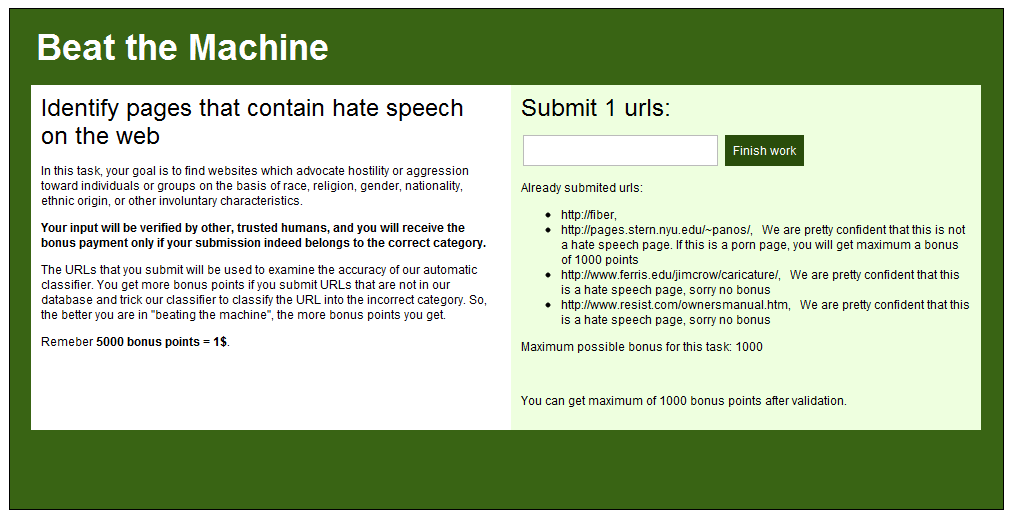
\includegraphics[width=\columnwidth]{plots/btm-HIT.png}}
\vspace{-.3in}
\caption{A screen-shot of the BTM interface on Mechanical Turk.}
\vspace{-.2in}
\label{fig:btm}
\end{figure}

\textbf{Segmenting the task by class}: To deal with these problems, we split the task into two subtasks: (1) Seek pages in the minority class that are misclassified in the majority class (i.e., pages that contain offensive content but are classified as benign), and (2) seek pages with benign content that would be classified as offensive. This segmentation simplified the overall design and made the task easier for participants to understand.  Moreover, it allowed us to quickly reject submissions that were of no interest.  For example, if we are asking for misclassified hate speech pages, we can quickly reject pages that our classifier unambiguously classifies as hate speech. (In the original design, users had the incentive to mark these as ``non-hate-speech'' hoping that the human judge would accept their judgments.) Figure~\ref{fig:btm} shows the (simple) task interface.

\textbf{Expanding the incentives}: In the final design (for this paper) we also improved the incentive structure by rewarding differently users that discover ``big mistakes'' (the ``unknown unknowns'') and those that discover the ``small mistakes'' (the ``known unknowns''). Instead of giving a constant bonus to the player for a misclassified URL, we reward misclassifications proportionally to the confidence of the classifier. 
If the model is not very confident of its classification of a submitted URL,
the reward is small.  This was a known unknown.
On the other hand, if the model is very confident in its decision (i.e., a classification confidence close to 100\%), but the decision is incorrect, then the BTM system gives the highest possible bonus to the worker.\footnote{In our particular implementation, the highest bonus is worth 1000 points, or 50 cents.} If the confidence was lower, say 75\%, then the reward was proportionally smaller. We also reward players that provide examples for which the model was correct but uncertain: if the model predicted that the page is 60\% likely to contain hate speech, and the page indeed contained hate speech, the user received a small bonus.





\section{Experimental Studies}

To provide a first experimental evaluation of BTM, we asked two questions:
\begin{itemize}

\item Does BTM identify errors efficiently?

\item Can we use the discovered errors to improve the models?

\end{itemize}

For our experiments, we used the BTM system to challenge two
classification systems. One for detecting pages with hate speech, and
one for detecting pages with adult content. We ran the systems with
the configuration details described in the previous section (1 cent
for the base task, 50 cents maximum payment for a URL that generates
an error).

\textbf{Comparison with stratified random testing:} For the two systems, we compared BTM with the usual quality assurance process of examining the output of the classifier to identify errors.  Examining a uniform random sample of the output is particularly uninformative, as the classifiers are quite accurate and the distributions are quite unbalanced, and so the vast majority of cases are correctly classified and not objectionable.  Therefore, standard procedure is to examine a random sample, stratified by the model's confidence score.  Specifically, the range of confidence scores [0,1] was divided into $k$ equal-width bins.  A set of $N$ URLs for testing was sampled randomly, with $\frac{N}{k}$ from each bin.  This stratification is used because it generally finds more errors, because it over-samples the URLs for which the models have low confidence (and are likely to be wrong).  However, the discovered errors are likely to be ``known unknowns.''  

For the adult classifier, the human workers identified errors in 16\% of the inspected cases (\textit{much} higher than the natural error rate of the classifier).  In contrast, using BTM, more than 25\% of the submitted cases generated an error (a 56\% increase). The corresponding statistics for hate speech were even better: workers identified errors only in 9\% of the inspections for stratified random sampling, but they identified errors in 27\% of the URLs with BTM. These results indicate that the BTM process is indeed more efficient than the standard evaluation procedure in identifying problematic cases.  It should be noted that we could increase the ``efficiency'' of the non-BTM procedure by simply sampling more from the low-confidence cases.  However, this would directly reduce the number of ``unknown unknowns'' discovered.  At the extreme, the largest number of errors would be found by sampling only in the low-confidence region.  All the errors found would then be known unknowns.  So, let's now consider the effect of BTM on the severity of the errors found.

\textbf{Comparing the severity of errors:} Figure~\ref{fig:hate-speech} and~\ref{fig:adult} show the distribution of errors for hate speech and adult content, respectively. A consistent behavior is observed for both categories: BTM identifies a significantly larger number of severe misses---the unknown unknowns. Within the errors identified by BTM, 25\% were cases of high severity; the model was confident that it was making the correct decision (classifying the content as benign, with 100\% confidence), but in reality the decision was incorrect. So, not only does BTM identify a larger number problematic cases than the stratified testing, but also a significant number of these cases were unknown unknowns: cases that would be missed and without a very unpleasant event (possibly a catastrophe), we never would know that we missed them. In contrast, and by now as expected, most of the identified 
errors for the stratified random sampling were near misses that occur near the decision boundary.

\begin{figure}[t]
\centering
\center{
\subfigure[Hate Speech]{
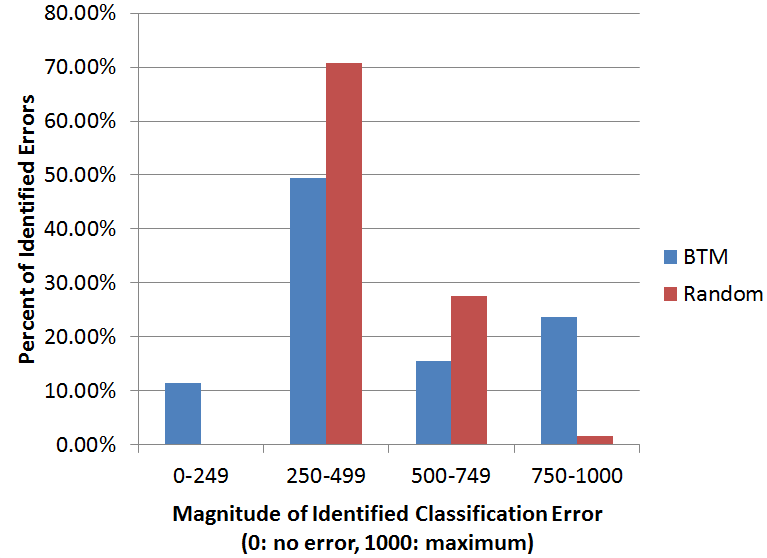
\includegraphics[width= \columnwidth]{plots/Hate-speech-scores.PNG}
\label{fig:hate-speech}
}
\subfigure[Adult Content]{
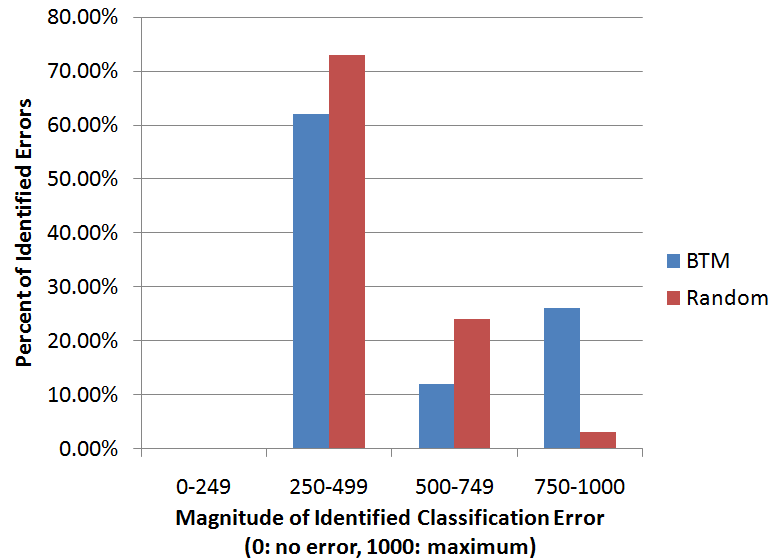
\includegraphics[width= \columnwidth]{plots/porn-scores.PNG}
\label{fig:adult}
}
\caption{Distributions of the magnitude of the identified errors by BTM and by random sampling for two ad safety tasks}
}
\label{fig:results}
\end{figure}

\drop{
\begin{figure}[t]
\center{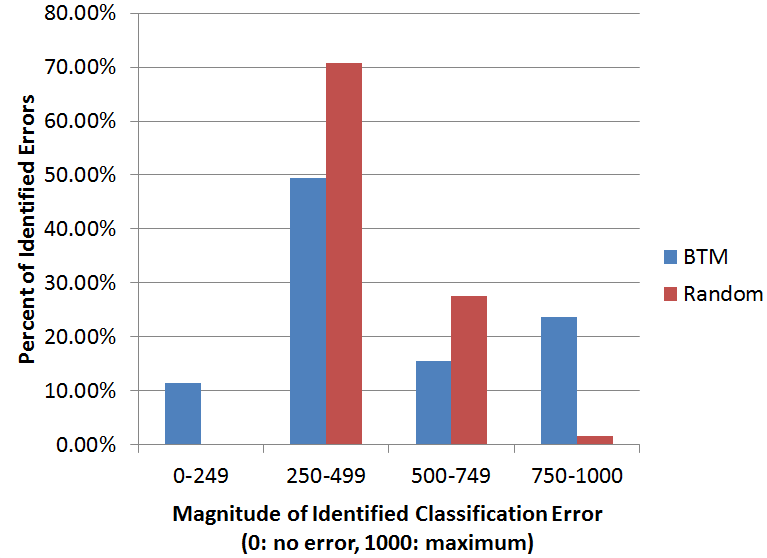
\includegraphics[width=\columnwidth]{plots/Hate-speech-scores.PNG}}
\caption{A distribution of the magnitude of the identified errors by BTM and by random sampling for the hate speech category.}
\label{fig:hate-speech}
\end{figure}

\begin{figure}[t]
\center{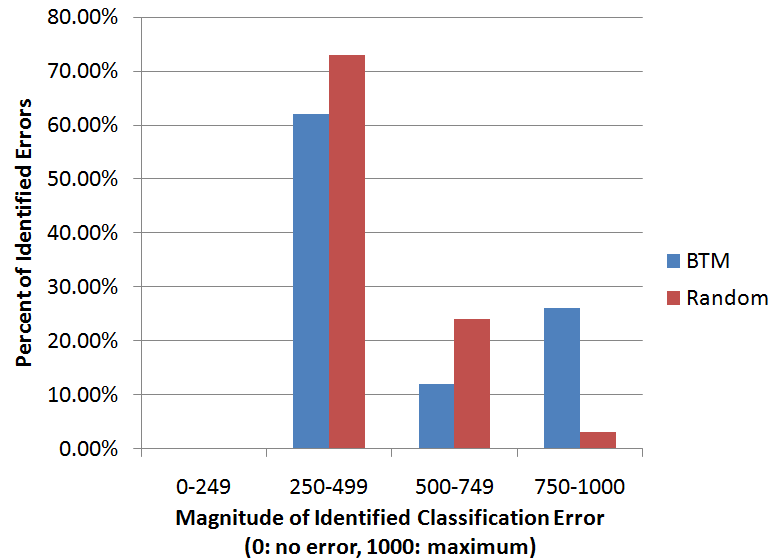
\includegraphics[width=\columnwidth]{plots/porn-scores.PNG}}
\caption{A distribution of the magnitude of the identified errors by BTM and by random sampling for the adult content category.}
\label{fig:adult}
\end{figure}
}

\textbf{Learning from identified errors:} The next, natural question is whether the identified erroneous decisions could be used to improve the decision models.  This actually is a very complicated problem, and a thorough treatment is beyond the scope of this short paper. For example, oversampling cases where a model makes big mistakes can be catastrophic for 
learning (think simply about oversampling outliers in a linear regression).
On the other hand, techniques like boosting \cite{Freund99ashort} have gotten tremendous
advantage by overweighting cases where the current model is incorrect.

Nevertheless, we can offer some initial insights. We can examine whether the cases found by BTM seem to be isolated outliers, or whether they seem to be regularities that can be modeled. To this end we ran the following experiment: We attempted to learn a model that would classify positive and negative examples from amongst the BTM-identified cases.\footnote{That is, false negatives and false positives from model being considered, respectively } Internal consistency in the identified errors would suggest that these cases are not outliers, but rather constitute parts of the space where the model fails systematically (potentially without being aware of the failures).

Figure~\ref{fig:curves} shows the results of this process. The ``btm only'' line shows the quality of the model built and tested using the error cases identified by the BTM process.  The ``student only'' line shows the quality of the model built and tested using examples gathered through stratified random sampling (the pages selected through random sampling were inspected by students, hence the name). Both the btm-only and student-only lines show quality measurements computed via cross-validation.  The results show that the quality of the models is fairly high, illustrating that there is consistency and internal coherence in these sets pages.  The fact that the BTM model can reach high levels of accuracy indicates that BTM indeed identifies systematic errors, and not just disparate outliers.  The comparatively lower quality of the random sampling model also illustrates that these pages are inherently more difficult to learn from; this is consistent with our discussion above that the discovery via stratified random sampling (DVSRS) focuses on the ambiguous cases (those that the current model is uncertain about), while BTM discovers incorrectly classified areas of the space that have been systematically ignored.

We also can examine whether the two approaches (DVSRS and BTM) identify sets of similar examples, or whether each of them identifies something completely different. For that, we tested the performance of BTM using the examples from DVSRS (``student'') and vice versa. The results indicate that there is little cross-consistency between the models. What we discover using BTM has little effectiveness on the error cases identified through DVSRS, and vice versa. This finding indicates  that BTM reveals errors in parts of the space unexplored by DVSRS.

BTM and DVSRS seem to be different processes, capable of identifying different types of errors. Each of these has its place in the evaluation and improvement of automatic models. DVSRS identifies cases where the model already knows that it is not confident. The BTM process, through its game-like structure and probing nature, encourages the discovery of unknown problems in the model. The fact that humans can easily find challenging cases for the automatic models, when being themselves confronted with this challenge, also indicates that human expertise and curiosity can improve even very accurate automatic models.



\begin{figure}[t]
\center{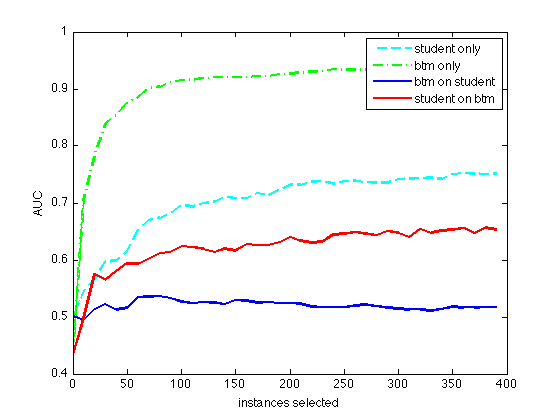
\includegraphics[width=\columnwidth]{plots/adt_btm_eval.png}}
\caption{Learning curves generated by the models
using cross-validation (BTM and student lines), and then use as test case for BTM the errors identified by random sampling (BTM on students), and vice versa (students on BTM).}
\label{fig:curves}
\end{figure}




\section{Current and Future Research}

We discussed and explored the design of the \emph{Beat the Machine} process for directly integrating humans into testing automatic decision models for vulnerabilities. Our results suggest that BTM is especially good in identifying cases where the model fails, while being confident that it is correct.  It is naturally interesting to examine how to best use knowledge of such vulnerabilities to improve the automatic decisions models. 


Vulnerability testing is common in areas of computer security, where ``white hat'' hackers with the appropriate expertise try to expose vulnerabilities in the security infrastructure of a firm. In our setting, we see that even lay users can easily find unknown holes in automatic decision models that test very well in ``standard'' tests, and show high classification performance when measured with the traditional, usual metrics (accuracy, AUC, etc).  Thus, builders of automatic decision models should take extra care when using these
traditional metrics for evaluations.

In our live deployment, untrained humans, with the appropriate incentives, were able to ``beat the machine'' seemingly easily, and discover a large number of vulnerabilities. This is, of course, useful by itself: the ``unknown unknowns'' become ``known unknowns'' and we can prepare to deal with these cases. But the key question for future research is also: how can we best incorporate such knowledge so that both ``unknown unknowns'' and ``known unknowns'' become ``known knowns.''

\section*{Acknowledgements}

The authors thank George A. Kellner and NEC for faculty fellowships,
and AdSafe Media for expertise, support, and data.  The models used in
this paper are not necessarily models used in production by any
company. This work was partially supported by the National Science 
Foundation under Grant No. IIS–0643846.


% [Add ambiguity in target variable to Limitations]

% ***To add to current/future work below:

%- How can we actually improve models with these unknown unknown cases?
%  Just plunking them into a training set yields mixed results.  This
%  may be because the training gets skewed, and we need to have a
%  specially designed training system.  Or it may be because we do not
%  really know how to evaluate the ``improved'' system.  What should be
%  the composition of the test set exactly?

%- In KDD-2010 we introduced guided learning, and showed that it can be
%  very useful for quickly building models in domains such as this.  We
%  are in the process of performing a similar comparison of BTM to GL.
%  Notably, GL also is not focused at all on the hard-to-envision
%  cases; in contrast, the incentive system there is to give easy to
%  find cases.

% For discussion:

% - relate to scenario planning
% - relate to white-hat hackers


\small{
\bibliographystyle{aaai}
\bibliography{activeinference} 
}


\end{document}